\documentclass {llncs}
\usepackage{tabularx,colortbl}
\usepackage[dvipsnames]{xcolor}
\usepackage{flushend}
\usepackage{cite}
\usepackage{amsmath}
%\usepackage{amsthm}
\usepackage{amssymb}
\usepackage{epsfig}
\usepackage{stmaryrd}
\usepackage{url}
\usepackage{multirow}
\usepackage{latexsym}
%\usepackage{float}
\usepackage{graphics}
\usepackage{graphicx}
%\usepackage{enumitem}
\usepackage{comment}
\usepackage{longtable}
\usepackage{supertabular}
\usepackage{times}
\usepackage{listings}
\usepackage{subfigure} 
\usepackage{color}
\usepackage{balance}
\usepackage[ruled, vlined, linesnumbered]{algorithm2e}
\usepackage{caption} \captionsetup[table]{skip=6pt}
%\usepackage{subcaption}


%\theoremstyle{Definition}
%\newtheorem{definition}{Definition}
%
%\theoremstyle{Theorem}
%\newtheorem{theorem}{Theorem}


%\newcommand{\definition}{\noindent \textbf{Definition} \citation{}}
%newcommand{\theorem}{\noindent \textbf{Theorem} \citation{}}


\newcommand{\mkeyword}[1]{\mbox{\texttt{#1}}}
\DeclareMathOperator{\kuop}{uop}
\DeclareMathOperator{\kbop}{bop}
\DeclareMathOperator{\kite}{ite}
\DeclareMathOperator{\kpre}{pre}
\DeclareMathOperator{\dom}{dom}
\DeclareMathOperator{\ktrue}{true}
\DeclareMathOperator{\kfalse}{false}
\DeclareMathOperator{\kselect}{select}
\DeclareMathOperator{\ran}{range}
\newcommand{\lbb}{[\![}
\newcommand{\rbb}{]\!]}
\newcommand{\expr}{\phi} 
\newcommand{\exprS}{\Phi}
% this toggles between a tech-report version of the paper and the MEMOCODE version
%\newcommand{\TECHREPORT}{}
%\tolerance=1
%\emergencystretch=\maxdimen
%\hyphenpenalty=10000
%\hbadness=10000
\sloppypar



\begin{document}

 % Add this to every tex file, so that you can comment with a diff color%
 \definecolor{gold}{rgb}{0.90,.66,0}
 \definecolor{dgreen}{rgb}{0,0.6,0}
\newcommand{\mike}[1]{\textcolor{red}{}}
\newcommand{\fixed}[1]{\textcolor{red}{#1}}
\newcommand{\ela}[1]{\textcolor{purple}{Ela: #1}}
\newcommand{\stateequiv}{\equiv_{s}}
\newcommand{\traceequiv}{\equiv_{\sigma}}

%\newcommand{\TECHREPORT}{}


\title{Experimental Evaluation of Set of Support %\thanks{This work has been supported by XXX}
}

\author{Elaheh Ghassabani\inst{1}, Andrew Gacek\inst{2}, and Michael W. Whalen\inst{1}}

\institute{Department of Computer Science and Engineering\\
 University of Minnesota, 200 Union Street, Minneapolis, MN 55455,USA\\
\email{\{whalen,ghassaba\}@cs.umn.edu}
 \and
Rockwell Collins Advanced Technology Center\\
400 Collins Rd. NE, Cedar Rapids, IA, 52498, USA\\
\email{\{andrew.gacek\}@rockwellcollins.com}
}

\maketitle

\begin{abstract}
Symbolic model checkers can construct proofs of properties over very complex models.  However, the results reported by the tool when a proof succeeds do not generally provide much insight to the user.  It is often useful for users to have traceability information related to the proof: which portions of the model were necessary to construct it.  This traceability information can be used to diagnose a variety of modeling problems such as overconstrained axioms and underconstrained properties, and can also be used to measure {\em completeness} of a set of requirements over a model.  In this paper, we present a new algorithm to efficiently compute the set of support within a model necessary for inductive proofs of safety properties for sequential systems.  The algorithm is based on the UNSAT core support built into current SMT solvers and a novel encoding of the inductive problem to try to generate a minimal set of support.  We prove our algorithm correct, and describe its implementation in the jkind model checker for Lustre models.  We then present an experiment in which we benchmark the algorithm in terms of speed, robustness, and minimality, with promising results.


\end{abstract}

%\keywords{Auto-traceability, Set of Support, Completeness, Requirement Engineering}

%\subsection{Experiment}
%\label{sec:experiment}

\newcommand{\takeaway}[1]{
\vspace{6pt}
\noindent\fbox{\parbox{0.975\columnwidth}{#1}}
\vspace{6pt}
}
 the overhead
in discovering all IVCs is a linear in the number of unique IVC
in the problem multiplied by the cost for finding a proof for
%\mike{What do we want to call our efficient algorithm: IVC?}

%We would like to investigate both the {\em efficiency} and {\em
%  minimality} of our three algorithms: the naive brute-force
%algorithm (\bfalg), the UNSAT core-based algorithm (\ucalg), and the
%combined UNSAT core followed by brute-force minimization algorithm
%(\ucbfalg). Efficiency is computed in terms of wall-clock time: how
%much overhead does the IVC algorithm introduce? Minimality is
%determined by the size of the IVC: cores with a smaller number of
%variables are preferred to cores with a larger number of variables.
%Finally, we are interested in the {\em diversity} of solutions: how
%often do different tools/algorithms generate different minimal IVCs?
%
%The use of \texttt{JKind} allows additional dimensions to our investigation: it supports two different inductive algorithms: $k$-induction and PDR, and a ``fastest'' mode, that runs both algorithms in parallel.  In addition, \texttt{JKind} supports multiple back-end SMT solvers including Z3~\cite{DeMoura08:z3}, Yices~\cite{Dutertre06:yices}, MathSAT~\cite{Cimatti2013:MathSAT}, and SMTInterpol~\cite{Christ2012:SMTInterpol}.  We would like to determine whether the choice of inductive algorithm affects the size of the IVC, whether different solvers are more or less efficient at producing IVCs, and whether running different solvers/algorithms leads to {\em diversity} of IVC solutions.
%
%Therefore, we investigate the following research questions:
%\begin{itemize}
%    \item \textbf{RQ1:} How expensive is it to compute inductive validity cores using the \bfalg, \ucalg, and \ucbfalg algorithms?
%    \item \textbf{RQ2:} How close to minimal are the IVC sets computed by \ucalg as opposed to the (guaranteed minimal) \ucbfalg?  How do the sizes of IVCs compare to static slices of the model?
%    \item \textbf{RQ3:} How much {\em diversity} exists in the solutions produced by different solver/induction algorithm configurations?
%\end{itemize}
%
%\subsection{Experimental Setup}
%In this study, we started from a suite of 700 Lustre models developed
%as a benchmark suite for~\cite{Hagen08:FMCAD}. We augmented this suite
%with 81 additional models from recent verification projects including
%avionics and medical devices~\cite{QFCS15:backes,hilt2013}. Most of
%the benchmark models from~\cite{Hagen08:FMCAD} are small (10kB or less,
%with 6-40 equations) and contain a range of hardware benchmarks and
%software problems involving counters. The additional models are much
%larger: around 80kB with over 300 equations. We added the new
%benchmarks to better check the scalability for the tools, especially
%with respect to the brute force algorithm.
%%
%%\mike{MORE HERE...stats on size, reasons for add'l models.}
%Each benchmark model has a single property to analyze.  For our purposes, we are only interested in models with a {\em valid} property (though it is perhaps worth noting that there is no additional computation---and thus no overhead---using the \texttt{JKind} IVC options for {\em invalid} properties).  In our benchmark set, 295 models yield counterexamples, and 10 additional models are neither provable nor yield counterexamples in our test configuration (see next paragraph for configuration information).  The benchmark suite therefore contains 476 models with valid properties, which we use as our test subjects.
%
%For each test model, we computed \ucalg in 12+1 configurations: the
%twelve configurations were the cross product of all solvers \{Z3,
%Yices, MathSAT, SMTInterpol\} and inductive algorithms
%\{$k$-induction, PDR, fastest\}, and the remaining (+1) configuration
%was an instance of \bfalg run on Yices, which is the default solver in
%\texttt{JKind}. In addition, for each of the 12 configurations, we ran an
%instance of \texttt{JKind} without IVC to examine overhead. The experiments
%were run on an Intel(R) i5-2430M, 2.40GHz, 4GB memory machine, with a
%1 hour timeout for each analysis on any model. The data gathered for
%each configuration of each model included the time required to check
%the model without IVC, with IVC, and also the set of elements in the
%computed IVC.\footnote{The benchmarks, all raw experimental results,
%  and computed data are available on \cite{expr}.}
%
%Note that not all analysis problems were solvable with all algorithms: for all solvers, $k$-induction (without IVC) was unable to solve 172 of the examples.  When comparing minimality of different solving algorithms, we only considered cases where both algorithms provided a solution (as will be discussed in more detail in Section~\ref{sec:minimality}).
%
%\iffalse
%\begin{itemize}
%    \item an algorithm to compute a truly minimal set of support, i.e. \texttt{JSupport}.
%    \item given a LUS model, a static crawler which automatically marks all equations of a node in the initial support set of a property.
%    \item some trackers that measure the verification time with/ without support computation.
%   % \item some minor changes in the XML writers.
%\end{itemize}
%
%\mike{My thoughts on this section: mostly, it needs more structure: more information on the properties of the models: size, provenance, etc., a broken out subsection on the description of the experimental setup, etc}
%
%\mike{I think we want to split out the results in another top-level section}
%
%Experiment:
%\begin{itemize}
%    \item (Overview) describe research questions and goals.
%    \item Experimental setup: tell me about the models: how many, how big are they?  Then, tell me about the experiment: the tool configurations, the machine used for test.
%    \item Data generation: Describe what you measured for each model analysis.
%\end{itemize}
%\fi
%
%
%%%  LocalWords:  minimality ive UNSAT IVC Minimality IVCs PDR Yices
%%%  LocalWords:  MathSAT SMTInterpol RQ JSupport


\section{Evaluation}
\label{sec:eval}
This section evaluates our approach by addressing the following research questions:

\ela{could you please rephrase these questions?! having hard time saying them clearly :-( }
\begin{itemize}
    \item \textbf{RQ1:} How much overhead does computation of set of support add to the proofs? 
    \item \textbf{RQ2:} How dependent is our approach on different tools and proof engines? Does different solvers/ proof engines generate different support set? If so, to what extent are they different?
    \item \textbf{RQ3:} Is there any relationship between the size of a computed support set and 
    solvers/ proof engines? 
    \item \textbf{RQ4:} Is there any relationship between the size of the model and the variety of support sets?
    \item \textbf{RQ5:} How close to minimal are the support sets computed by our algorithm? For each model, we have 12 sets of support computed by \texttt{JKind}, and one \emph{minimal} set computed by \texttt{JSupport}; we would like to know which configurations generated sets that are very close or far to the minimal one.
    \item \textbf{RQ6:} How do different solvers perform on computing support? And, how efficient is it in comparison with \texttt{JSupport}?
\end{itemize} 

\subsection{Analytical Results}
\label{sec:res}
This section answers the aforementioned research questions briefly describing the way the results are analyzed. Note that the results of 10 models with unprovable properties are omitted in calculations. In addition, while analyzing support sets, \texttt{K-induction} settings that timed out were not considered because they failed to prove the properties. 

In general, for timing analyses, from all 13 configurations, we only considered the settings where both \texttt{PDR} and \texttt{K-induction} engines were activated. Since this configuration is a default setting in \texttt{JKind}, we only care about timing while both engines are employed. Therefore, $(4 \times 405) = 1620$ of all 5265 runs have been analyzed to address time-efficiency questions.


% RQ1: the overhead of support computation on different solvers
\textbf{RQ1.} The overhead is defined as the percentage of the overall runtime is dedicated to support computation:

\mbox{$overhead\_percentage = 100 \times (support\_runtime \div overall\_runtime)$}

 Table~\ref{tab:overhead} shows the overhead of support computation on different solvers.


\begin{table}
  \centering
  \begin{tabular}{ |c||c|c|c|c| }
    \hline
     solver & min & max & mean & stdev \\[0.5ex]
    \hline
    Z3   & 0.726\% & 45.396\% & 13.414\% & 11.369\% \\[0.5ex]
    Yices &   0.200\%  & 262.254\%   & 47.264\% & 51.193\% \\[0.5ex]
    SMTInterpol& 0.930\% & 268.571\% &  70.500\% & 58.541\%\\[0.5ex]
    MathSAT & 0.502\% & 396.124\% &  71.007\% & 79.990\%\\[0.5ex]
    \hline
  \end{tabular}
  \caption{\small{Overhead of support computation on different solvers}}
  \label{tab:overhead}
\end{table}

\vspace{6pt}
\noindent\fbox{%
    \parbox{\textwidth}{%
        In average, computation of support set has less than 50\% overhead. Averagely, if it takes \textit{t} to prove $\mathbb{P}$, it will take \textit{1.5t} to both prove $\mathbb{P}$ and compute its set of support.
    }%
}
 \vspace{9pt}

% RQ2: How dependent is our approach on different tools and proof engines?
\textbf{RQ2.} To answer this question, we analyzed the results from different aspects. The following describes methods used for analyzing and their results.

\textbf{(1)} For each model in the benchmark, the experiments generated 13 different sets of support. We used Jaccard distance to measure dissimilarity between pairwise of these sets:

\begin{center}
$d_J(\small{A}, \small{B}) = 1 - \frac{|A \cap B|}{|A \cup B|} ,\hspace{9pt} 0 \leq d_J(\small{A}, \small{B}) \leq 1$
\end{center}
\vspace{6pt} 

Therefore, we obtained $\binom{13}{2} = 78$ combinations of distances per model. Then, minimum, maximum, average, and standard deviation of the distances were calculated (Fig~\ref{fig:jacdis}), by which, again, we calculate these four measures among all 405 models. The following summarizes the result of this analysis:
\begin{itemize}
  \item Minimum Jaccard distance among all models is: 0.0 
  \item Maximum Jaccard distance among all models is: 0.882 
  \item Average Jaccard distance among all models is: 0.027 
  \item Standard deviation of Jaccard distance among all models is: 0.062 
\end{itemize}


\begin{figure}
  \centering
  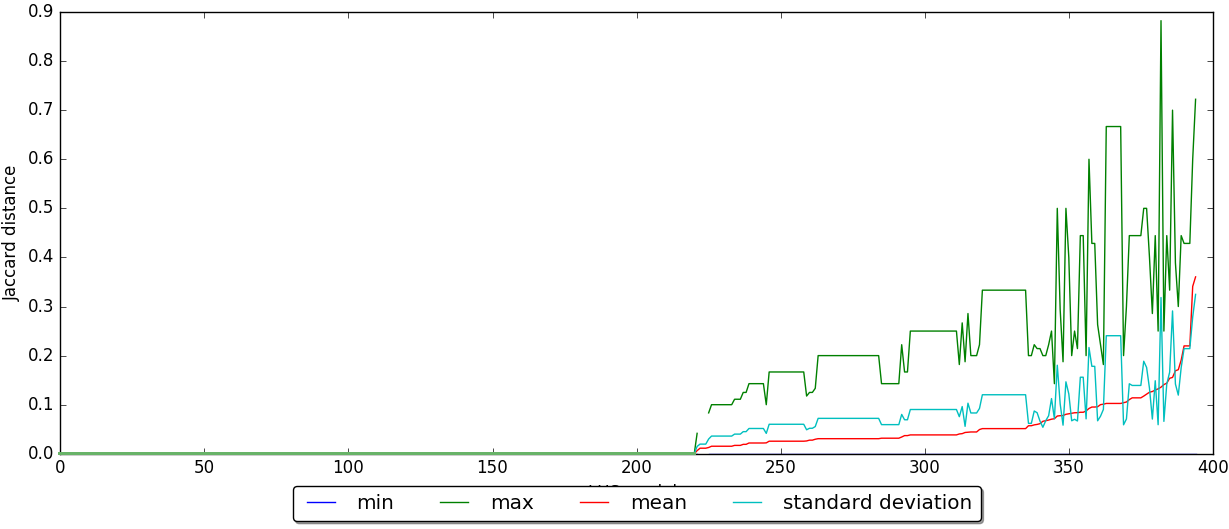
\includegraphics[width=\textwidth]{figs/jacdis.png}
  \caption{\small{Pairwise Jaccard distance between support sets}}\label{fig:jacdis}
\end{figure}

\vspace{6pt}
\noindent\fbox{%
    \parbox{\textwidth}{%
        Support sets computed with different solvers and engines have an average Jaccard distance of 0.027, which implies our algorithm has very small dependency on tools and proof algorithms.
    }%
}
 \vspace{9pt}
 
\textbf{(2)} Since one goal was to know to what extent computed support sets are different, and which configurations have generated more different/similar sets. We analyzed the results,
and it turns out 174 models of 405 contain at least two different support sets (which means in 231 models, all 13 sets of support are the same). We analyzed those 174 models; for each of them, pairwise Jaccard distance between sets was compared, and configurations with maximum/ minimum distances were collected. Fig~\ref{fig:maxdis} and Fig~\ref{fig:mindis} show the results. For example, in Fig~\ref{fig:maxdis}, in 20 models out of 405, \texttt{JSupport} and the configuration where \texttt{Z3} and both proof engines were employed, Jaccard distance between support sets computed by them is maximum. As you can see, different configurations of \texttt{JKind} do not affect very much the variety of the generated sets. However, \texttt{JSupport} and \texttt{JKind} configurations have had maximum distances most of the time. Even so, the frequency of such maximum distances among 405 models is very low.


\begin{figure}
  \centering
  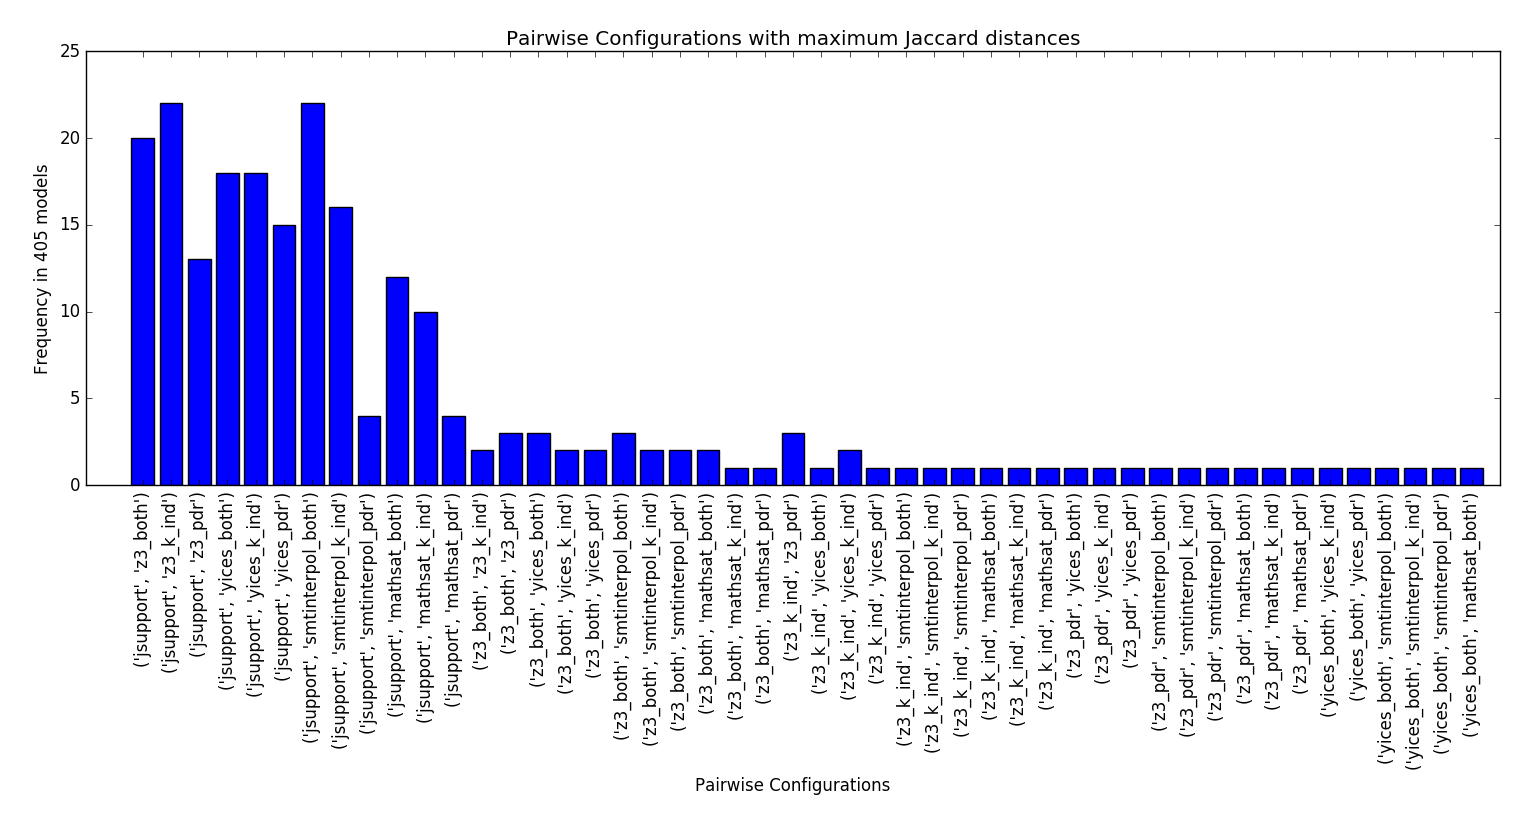
\includegraphics[width=\textwidth]{figs/max_settings_analyses.png}
  \caption{\small{Pairwise configurations with maximum Jaccard distance}}\label{fig:maxdis}
\end{figure}


\begin{figure}
  \centering
  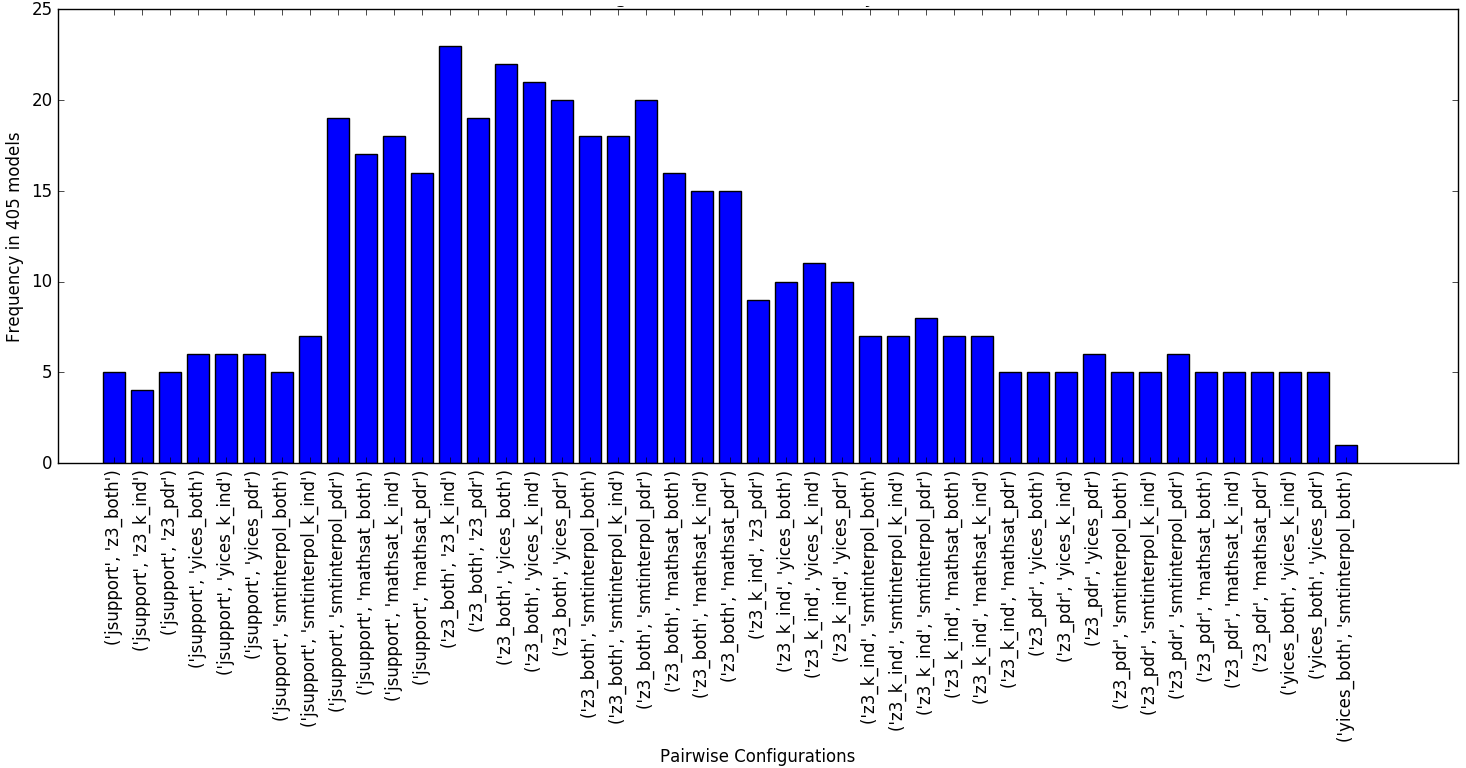
\includegraphics[width=\textwidth]{figs/min_settings_analyses.png}
  \caption{\small{Pairwise configurations with minimum Jaccard distance}}\label{fig:mindis}
\end{figure}

\vspace{6pt}
\noindent\fbox{%
    \parbox{\textwidth}{%
        Different solvers and proof engines have very small impact on the variety of elements in a support set of a property computed by our algorithm.
    }%
}
 \vspace{9pt}

\textbf{(3)} In addition to Jaccard distance, we also measured the similarity among all sets computed in different configurations per model. Let $S_M$ be a set of all support sets computed for model $M$ (i.e. in our experiments, $S_M$ is a set of 13 sets).  We define similarity per model as follows:

\begin{center}
$similarity = \frac{|\bigcap_{i=1}^{13} s_{Mi}|}{|\bigcup_{i=1}^{13} s_{Mi}|}, \hspace{9pt} s_{Mi} \in S_M$
\end{center}
\vspace{6pt} \ela{should see if this formula has any name in mathematics?!}

Needless to say, $0 \leq similarity \leq 1$, and if all the sets in $S_M$ are the same, \textit{similarity} will be 1. So the closer to 1 it is, the more similar sets we have. Fig~\ref{fig:sim} shows similarity in all models. Here is also a summary of minimum, maximum, average, and standard deviation of similarity among all models:
\begin{itemize}
  \item minimum similarity among all models is: 0.12
  \item maximum similarity among all models is: 1.0
  \item average similarity among all models is: 0.884
  \item standard deviation of similarity among all models is: 0.165
\end{itemize}


\begin{figure}
  \centering
  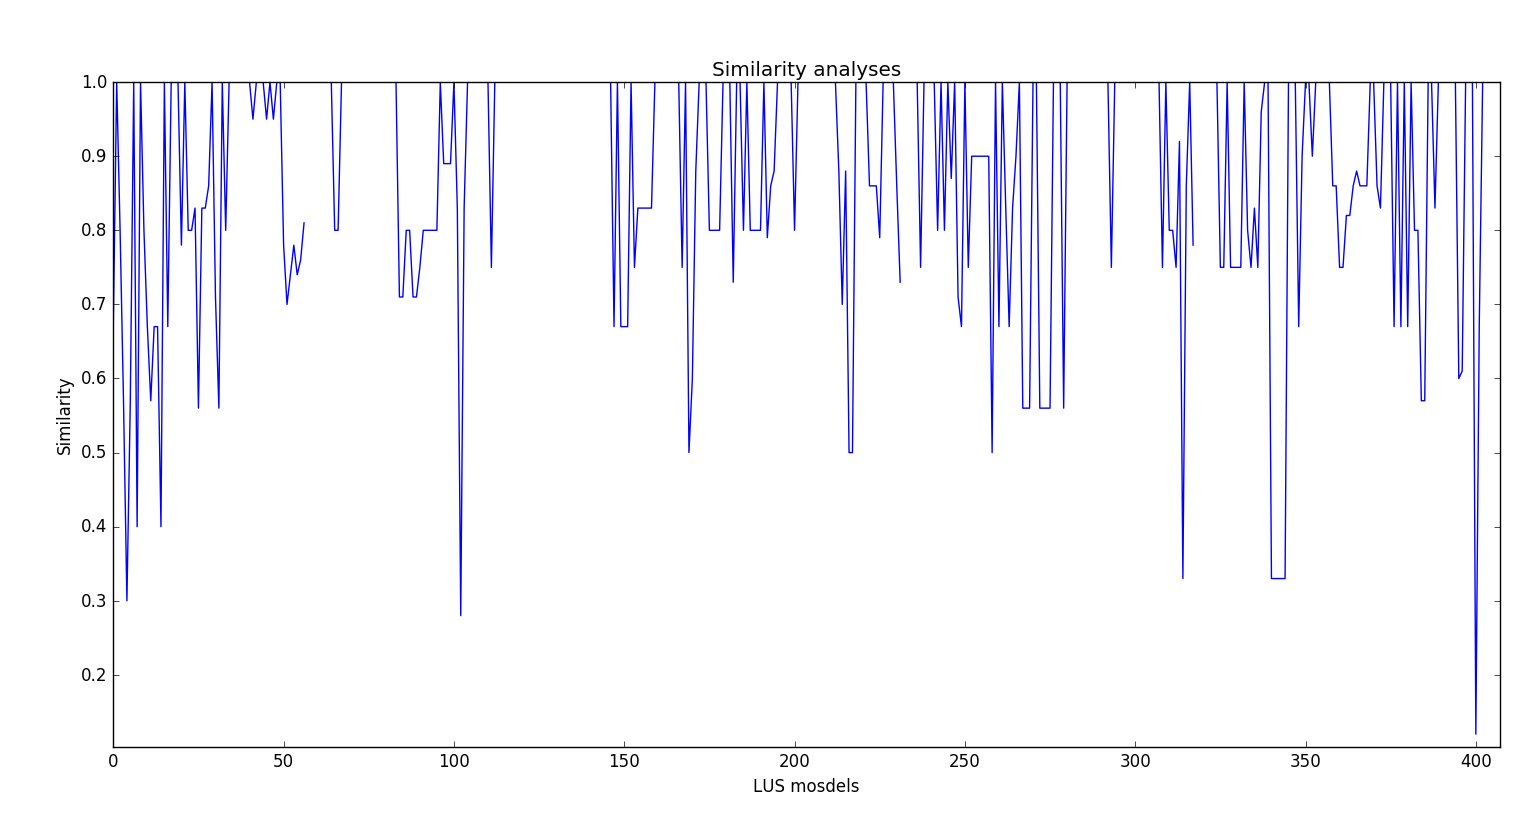
\includegraphics[width=\textwidth]{figs/similarity.png}
  \caption{\small{Similarity measurement for all models}}\label{fig:sim}
\end{figure}

\vspace{6pt}
\noindent\fbox{%
    \parbox{\textwidth}{%
        An average \textit{similarity} of 0.884 shows that support sets computed in different 
        configurations are very similar. So, the dependency of our algorithm to different solvers and proof engines is negligible.
    }%
}
 \vspace{9pt}

\textbf{(4)} We also calculated a \emph{core} support set for each model of the benchmark; A core set of model $M$ is defined as
$\bigcap_{i=1}^{13} s_{Mi},   \hspace{9pt} s_{Mi} \in S_M$. Then, the size difference of the core set with the smallest support set of $M$ was calculated. The results are visualized in Fig~\ref{fig:core}


\begin{figure}
  \centering
  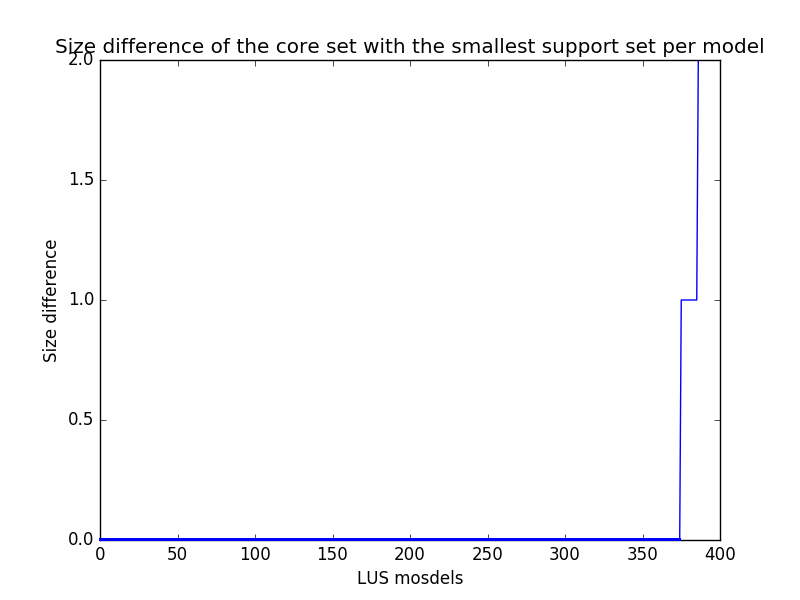
\includegraphics[width=\textwidth]{figs/core.png}
  \caption{\small{Size difference between the core set and the smallest support set per model}}\label{fig:core}
\end{figure}

\vspace{6pt}
\noindent\fbox{%
    \parbox{\textwidth}{%
        The core support set is very close to the smallest support set of a property.
    }%
}
 \vspace{9pt}

% RQ3: Is there any relationship between the size of a computed support set and
%solvers/ proof engines? 
\textbf{RQ3:} To address this question, we analyzed the raw data with two different approaches described in the following.
 
\textbf{(1)} We analyzed the sets of each 405 models. In each model, we looked for configurations that generated the biggest support set and ones that generated the smallest. Fig~\ref{fig:smallest} and Fig~\ref{fig:bigest} visualize the result of this analysis. For example, as you can see in Fig~\ref{fig:bigest}, \texttt{JSupport} generated biggest support sets in less than 10 models. Note that it implies there is at least one \texttt{JKind} configuration that generated the set with a smaller size.


\begin{figure}
  \centering
  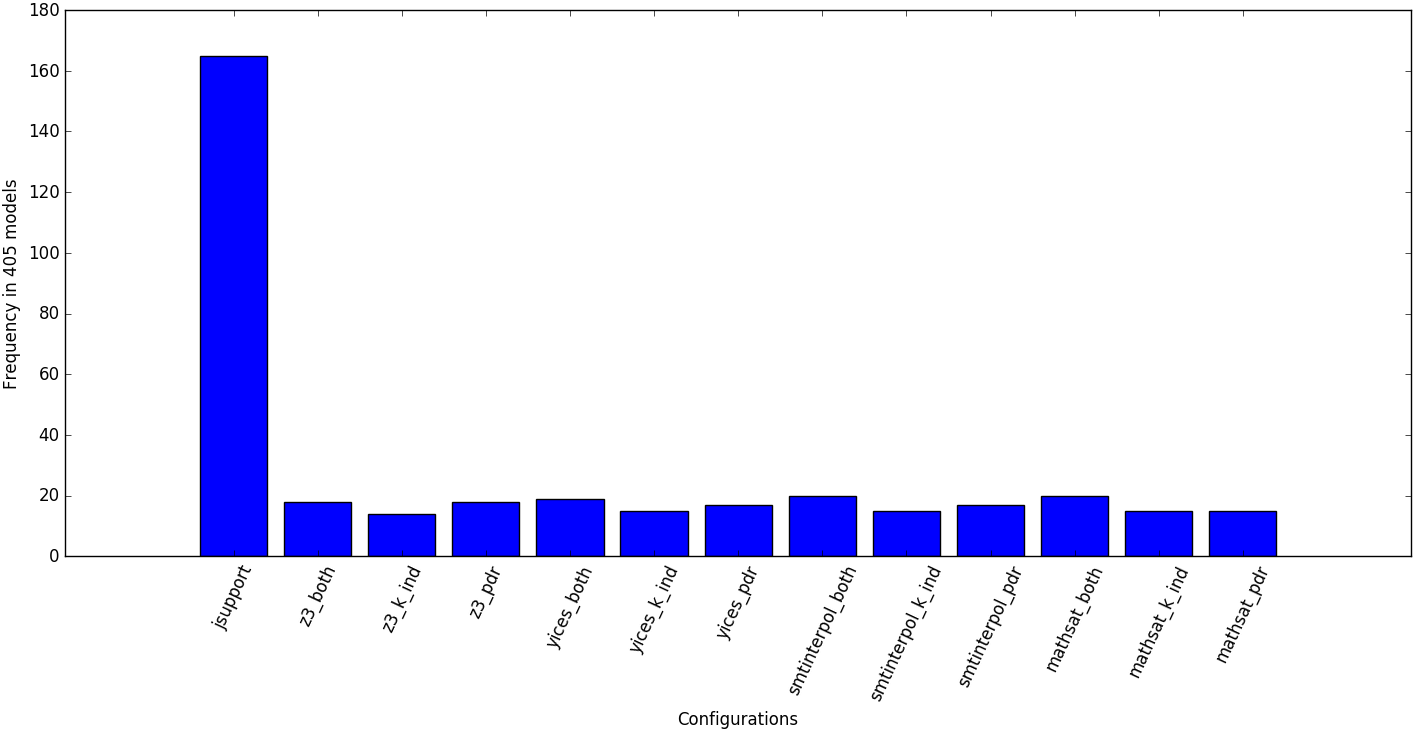
\includegraphics[width=\textwidth]{figs/small_conf.png}
  \caption{\small{Smallest support set (in terms of size) vs configurations}}\label{fig:smallest}
\end{figure}


\begin{figure}
  \centering
  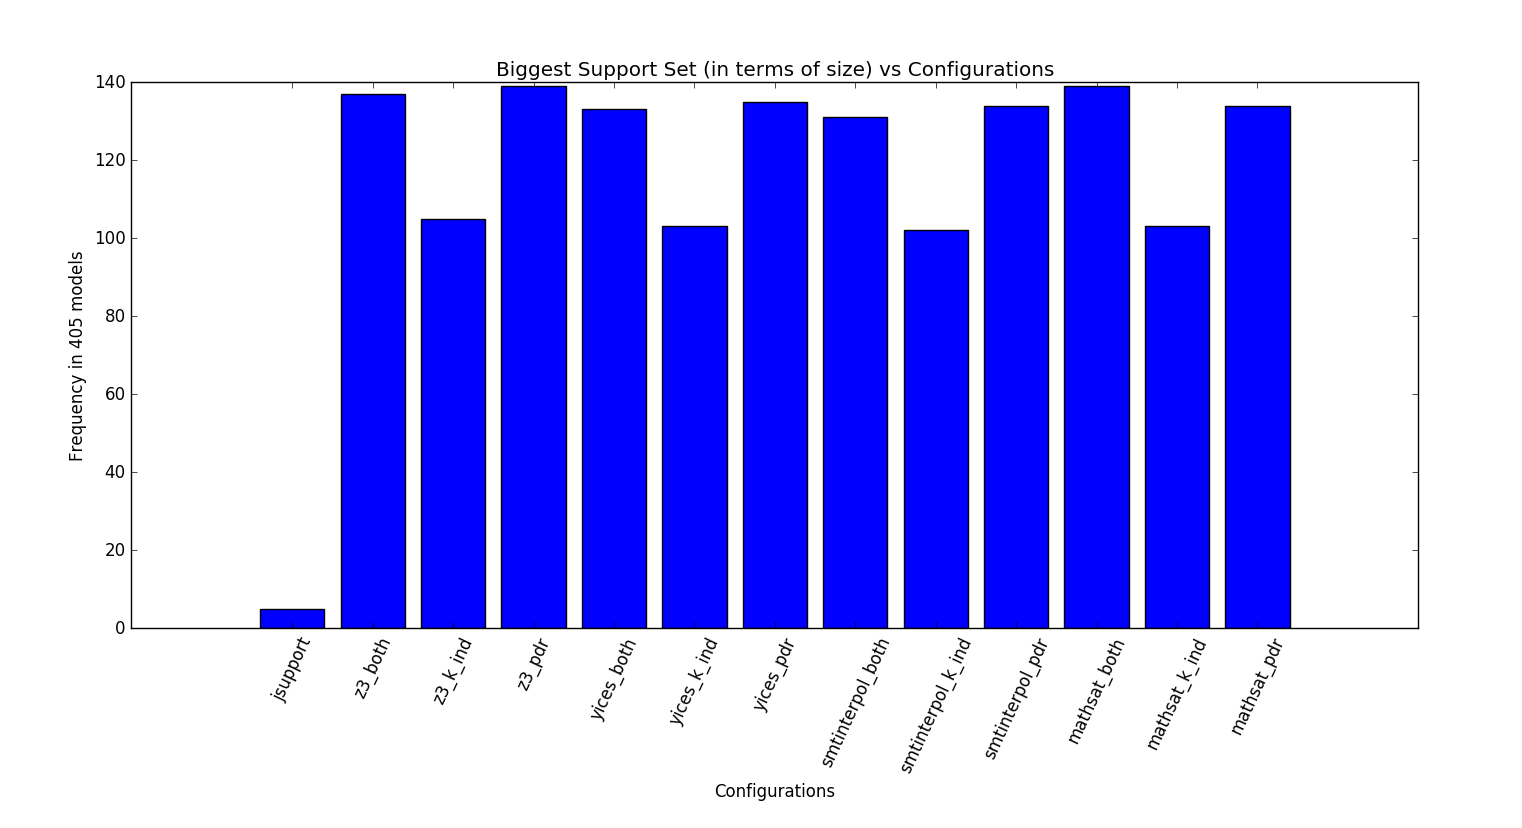
\includegraphics[width=\textwidth]{figs/big_conf.png}
  \caption{\small{Biggest support set (in terms of size) vs configurations}}\label{fig:bigest}
\end{figure}

\vspace{6pt}
\noindent\fbox{%
    \parbox{\textwidth}{%
    Solvers/ proof engines have negligible effects on the size of the support set computed by \texttt{JKind}.
    }%
}
 \vspace{9pt}

\textbf{(2)} Since \texttt{JSupport}, with a great percentage, most of the time computed the smallest support set, we compared the size of the sets computed in each \texttt{JKind} configuration with \texttt{JSupport} per model. Fig~\ref{fig:minpdr} to Fig~\ref{fig:minboth} represent the results. If we take a closer look at the results in the pictures, we can summarize them as shown in Table~\ref{tab:minimality}. For each configuration, we collected the difference between its support size and \texttt{JSupport} per model. Then, minimum, maximum, average, and standard deviation of the collected data have been reported.


\begin{figure}
  \centering
  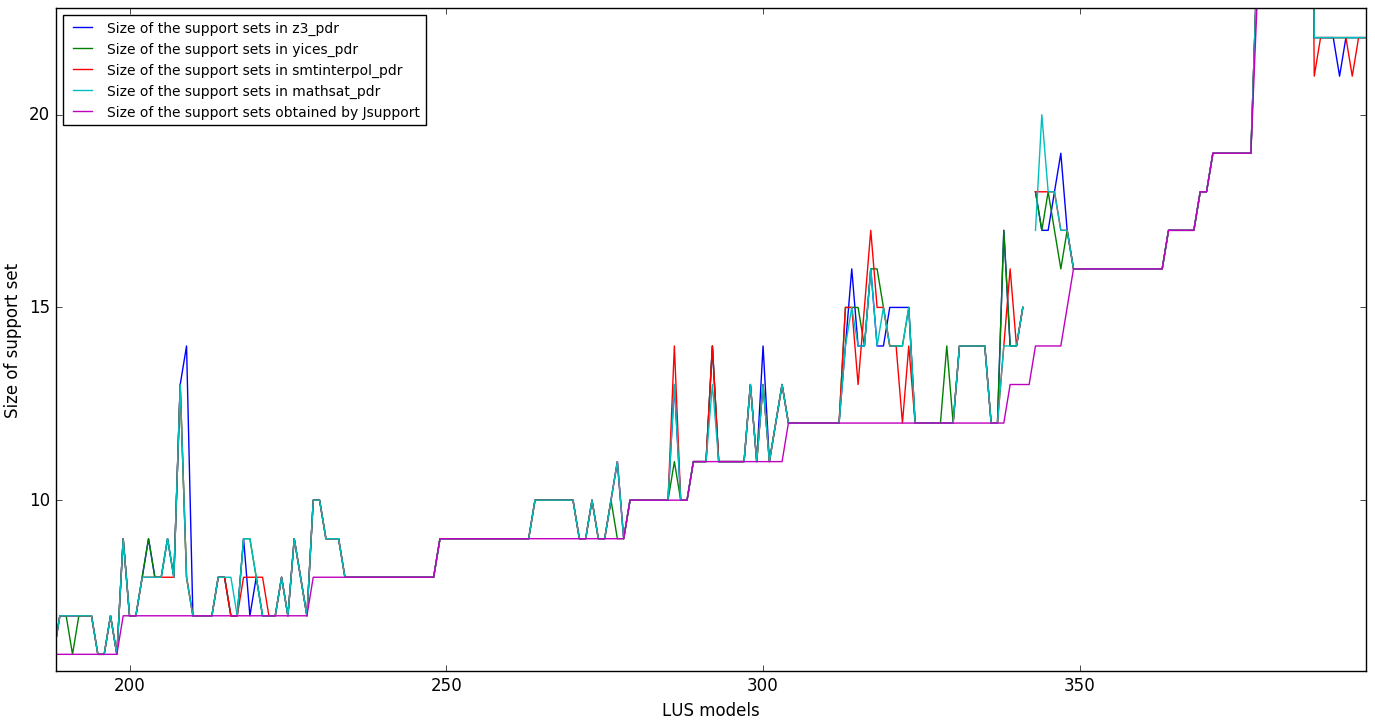
\includegraphics[width=\textwidth]{figs/minimality_pdr.png}
  \caption{\small{Minimality comparison of \texttt{PDR}}}\label{fig:minpdr}
\end{figure}


\begin{figure}
  \centering
  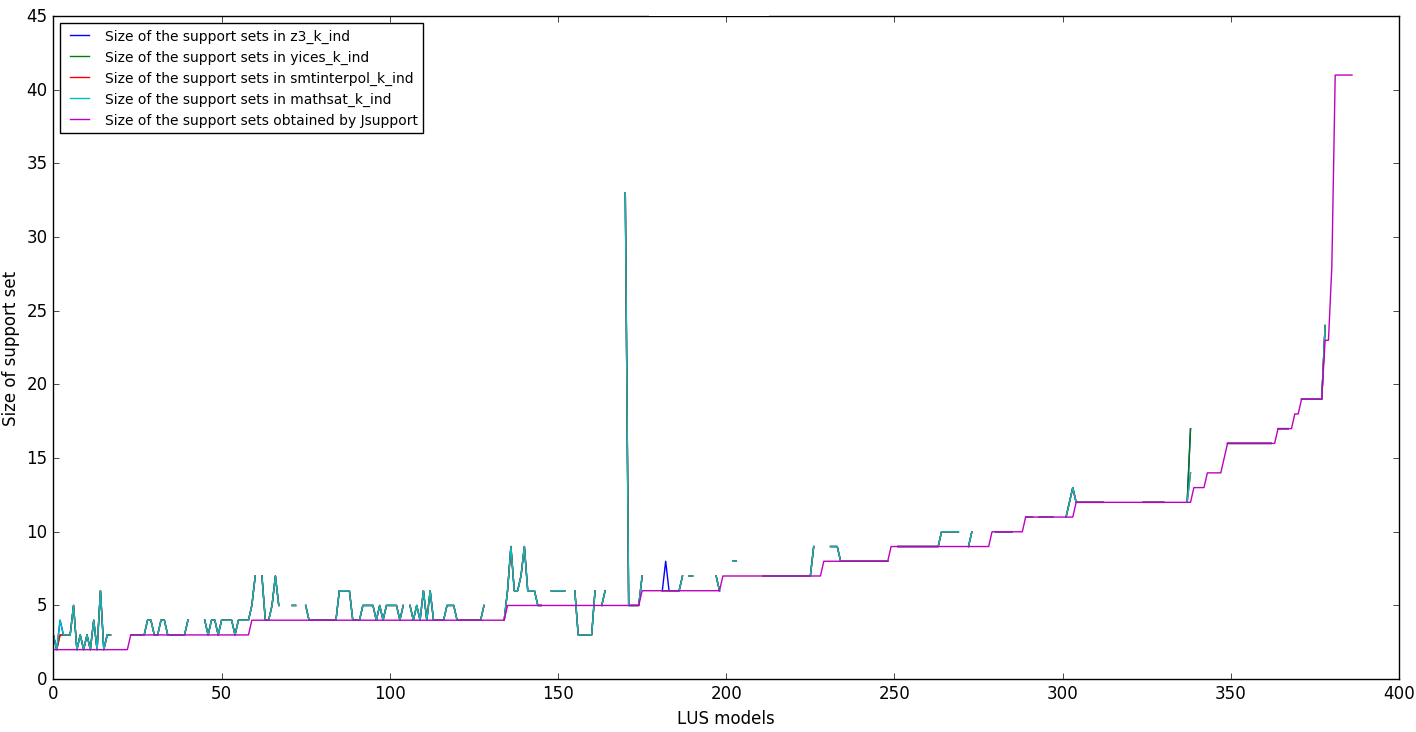
\includegraphics[width=\textwidth]{figs/minimality_kind.png}
  \caption{\small{Minimality comparison of \texttt{K-induction}}}\label{fig:minkind}
\end{figure}


\begin{figure}
  \centering
  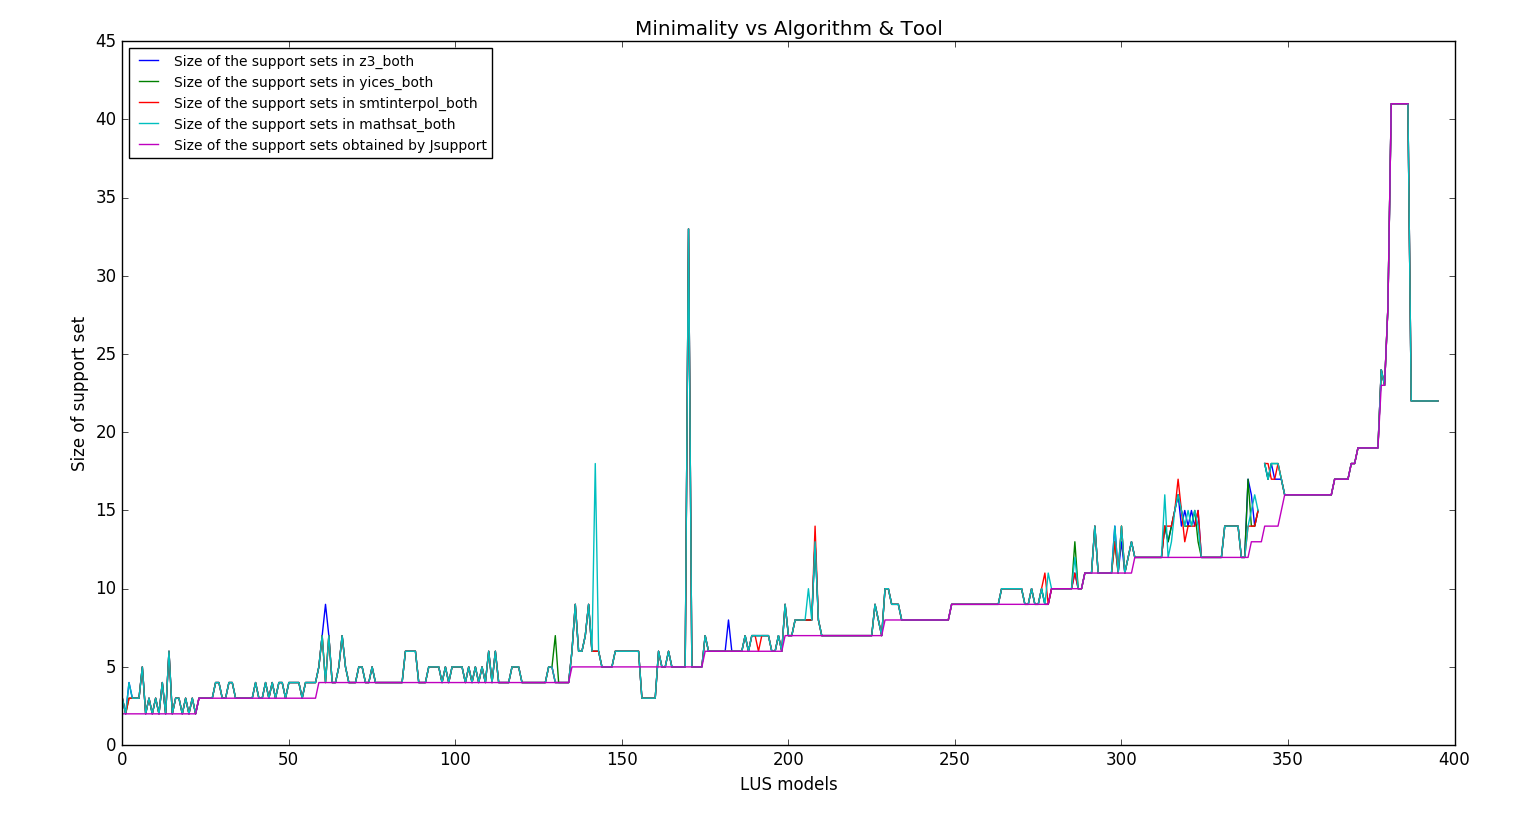
\includegraphics[width=\textwidth]{figs/minimality_both.png}
  \caption{\small{Minimality comparison of \texttt{K-induction} and \texttt{PDR} working together}}\label{fig:minboth}
\end{figure}


\begin{table}
  \centering
  \begin{tabular}{|c|c|c|c|c|}
     \hline
     configuration & min & max & mean & stdev \\[0.5ex]
     \hline\hline
     K-induction & -2 & 28 & 0.542 & 1.831 \\[0.5ex]
     PDR & -2 & 28 & 0.677 & 1.819 \\[0.5ex]
     Both engines & -2 & 28 & 0.661 & 1.751 \\[0.5ex]
     \hline
     Z3, K-ind & -2 & 28 & 0.555 & 1.842 \\[0.5ex]
     Yices, K-ind & -2 & 28 & 0.544 & 1.838 \\[0.5ex]
     SMTInterpol, K-ind & -2 & 28 & 0.534 & 1.822 \\[0.5ex]
     MathSAT, K-ind & -2 & 28 & 0.537 & 1.823 \\[0.5ex]
     \hline
     Z3, PDR & -2 & 28 & 0.697 & 1.852 \\[0.5ex]
     Yices, PDR & -2 & 28 & 0.668 & 1.807 \\[0.5ex]
     SMTInterpol, PDR & -2 & 28 & 0.673 & 1.813 \\[0.5ex]
     MathSAT, PDR & -2 & 28 & 0.668 & 1.803 \\[0.5ex]
     \hline
     Z3, Both engines & -2 & 28 & 0.663 & 1.729 \\[0.5ex]
     Yices, Both engines & -2 & 28 & 0.650 & 1.721 \\[0.5ex]
     SMTInterpol, Both engines & -2 & 28 & 0.637 & 1.713 \\[0.5ex]
     MathSAT, Both engines & -2 & 28 & 0.692 & 1.837 \\[0.5ex]
     \hline     
   \end{tabular}
  \caption{\small{Summary of minimality analyses}}\label{tab:minimality}
\end{table}

\vspace{6pt}
\noindent\fbox{%
    \parbox{\textwidth}{%
     \texttt{JKind} is able to find minimal support sets with a very negligible dependency on solvers/ proof engines.
    }%
}
 \vspace{9pt}

% RQ4: Is there any relationship between the model size and variety of its support sets?
\textbf{RQ4.} The size of the models in our benchmark is between 0 KB and 10 KB. 
We divided the models into 9 different categories based on their sizes such that $category_i$ contains
all models whose sizes are between $(i - 1)$ KB and $i$ KB. Then, using the \textit{similarity} formula defined in RQ2, the similarity for each model in each category was calculated. After that, minimum, maximum, average, standard deviation of the data were obtained per category. Table~\ref{tab:modelsize} summarizes the result of this analysis; the column \emph{number} in the table shows the number of models in each category, which means the sum of the numbers in the column is 405 (for example, there are 6 models whose sizes are between 8 KB and 9 KB, and in all of them \textit{similarity} is 1.0).
 
 
\begin{table}
  \centering
  \begin{tabular}{ |c||c|c|c|c|c|}
    \hline
    size (KB) & number&
     min & max & mean & stdev \\[0.5ex]
    \hline\hline
    [0-1] & 49 & 0.33 & 1.0 & 0.877 & 0.213 \\[0.5ex]
    [1-2] & 90& 0.3 & 1.0 & 0.835 & 0.192 \\[0.5ex]
    [2-3] & 26&0.5 & 1.0 & 0.876 & 0.131 \\[0.5ex]
    [3-4] & 34&0.57 & 1.0 & 0.896 & 0.158 \\[0.5ex]
    [4-5] & 88&0.12 & 1.0 & 0.895 & 0.153 \\[0.5ex]
    [5-6] & 11&0.75 & 1.0 & 0.83 & 0.107 \\[0.5ex]
    [6-7] & 2&0.96 & 1.0 & 0.98 & 0.02 \\[0.5ex]
    [7-8] & 99&0.28 & 1.0 & 0.916 & 0.124 \\[0.5ex]
    [8-9] & 6&1.0 & 1.0 & 1.0 & 0.0 \\[0.5ex]
    \hline
  \end{tabular}
  \caption{Model size vs similarity among its support sets}\label{tab:modelsize}
\end{table}

\vspace{6pt}
\noindent\fbox{%
    \parbox{\textwidth}{%
     The size of the model does not affect the stability of our algorithm; 
     if a model is large, it does not mean that it will have a lot of different minimal support sets. In other words, minimal support sets of a given property computed by \texttt{JKind} will be very similar to each other.
    }%
}
 \vspace{9pt}
 
% RQ5: How close to minimal are the support sets computed by our algorithm? For each model, we have 12 sets of support computed by \texttt{JKind}, and one \emph{minimal} set computed by \texttt{JSupport}; we would like to know which configurations generated sets that are very close or far to the minimal one.

\textbf{RQ5.} To address this question, we analyzed our experimental data from different viewpoints described in the following.

\textbf{(1)} We would like to know which configurations generated sets that are very close or far to the minimal one. To address this question, we calculated pairwise Jaccard distance between sets obtained from different configurations and \texttt{JSupport} per model. Then, minimum, maximum, mean, and standard deviation of the calculated data were obtained among all models. Fig~\ref{fig:jsupjadis} is a summary of this analysis. The result can be also summarized as follows:
\begin{itemize}
  \item minimum of Jaccard distances from \texttt{JSupport} among all models is: 0.0
  \item maximum of Jaccard distances from \texttt{JSupport} among all models is: 0.882
  \item standard deviation for Jaccard distances from \texttt{JSupport} among all models is: 0.034
  \item average of Jaccard distances from \texttt{JSupport} is: 0.103
\end{itemize}


\begin{figure}
  \centering
  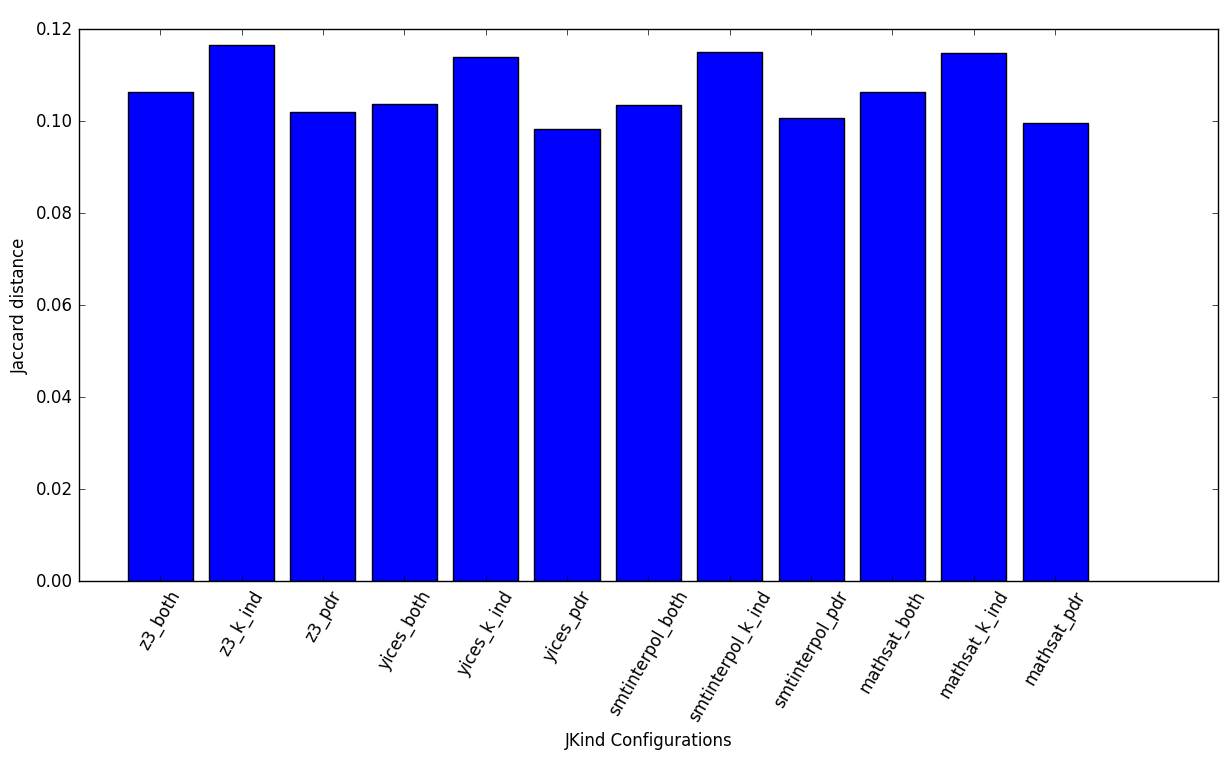
\includegraphics[width=\textwidth]{figs/jsupport_analyses.png}
  \caption{\small{Average Jaccard distance between \texttt{JSupport} and different configurations}}\label{fig:jsupjadis}
\end{figure}

\vspace{6pt}
\noindent\fbox{%
    \parbox{\textwidth}{%
    Using different solvers/ proof engines in \texttt{JKind} has negligible effect on the minimality of the support sets.
    }%
}
 \vspace{9pt}
 
\textbf{(2)} For 405 models, we calculated minimum, maximum, avgerage, and standard deviation of Jaccard distance between JSupport and each configuration
to see which configuration generates support sets close to minimal. 
Table~\ref{tab:jsupconf} represents the result of this analysis; for example, configuration \emph{(Z3, Both)}, shows that \texttt{JKind} with \texttt{Z3} and both \texttt{K-induction} and \texttt{PDR} engines has an average Jaccard distance of 0.106 (in 405 models) from \texttt{JSupport}.


\begin{table}
  \centering
  \begin{tabular}{|c|c|c|c|c|}
    \hline
    configuration & min & max & mean & stdev \\[0.5ex]
    \hline\hline
    Z3, Both & 0.0 & 0.882 & 0.106 & 0.155 \\[0.5ex]
    Z3, K-induction & 0.0 & 0.882 & 0.116 & 0.168 \\[0.5ex]
    z3, PDR & 0.0 & 0.882 & 0.102 & 0.151 \\[0.5ex]
    \hline
    Yices, Both & 0.0 & 0.882 & 0.104 & 0.152 \\[0.5ex]
    Yices, K-induction & 0.0 & 0.882 & 0.114 & 0.166 \\[0.5ex]
    Yices, PDR & 0.0 & 0.882 & 0.098 & 0.147 \\[0.5ex]
    \hline
    SMTInterpol, Both & 0.0 & 0.882 & 0.103 & 0.152 \\[0.5ex]
    SMTInterpol, K-induction & 0.0 & 0.882 & 0.115 & 0.167 \\[0.5ex]
    SMTInterpol, PDR & 0.0 & 0.882 & 0.101 & 0.149 \\[0.5ex]
    \hline
    MathSAT, Both & 0.0 & 0.882 & 0.106 & 0.156 \\[0.5ex]
    MathSAT, K-induction & 0.0 & 0.882 & 0.115 & 0.167 \\[0.5ex]
    MathSAT, PDR & 0.0 & 0.882 & 0.100 & 0.148 \\[0.5ex]
    \hline
  \end{tabular}
  \caption{\small{Jaccard distance between \texttt{JSupport} and each configuration}}\label{tab:jsupconf}
\end{table}

\vspace{6pt}
\noindent\fbox{%
    \parbox{\textwidth}{%
    Different configurations of \texttt{JKind} generated support sets that are very close to minimal sets computed by \texttt{JSupport}.
    }%
}
 \vspace{9pt}

\textbf{(3)} The next approach we took to address this question was to analyze the size of the biggest and smallest support sets versus \texttt{JSupport} per model. The results are shown in Fig~\ref{fig:minjsup}.
We computed the size of the biggest and smallest sets per model, then added them together for all models. The same calculation has been done for JSupport:
\begin{itemize}
  \item the aggregate number of elements in the \emph{smallest} support sets is : 3263
  \item the aggregate number of elements in the \emph{biggest} support sets is: 3609
  \item the aggregate number of elements in support sets computed by \texttt{JSupport} is: 3078
\end{itemize}


\begin{figure}
  \centering
  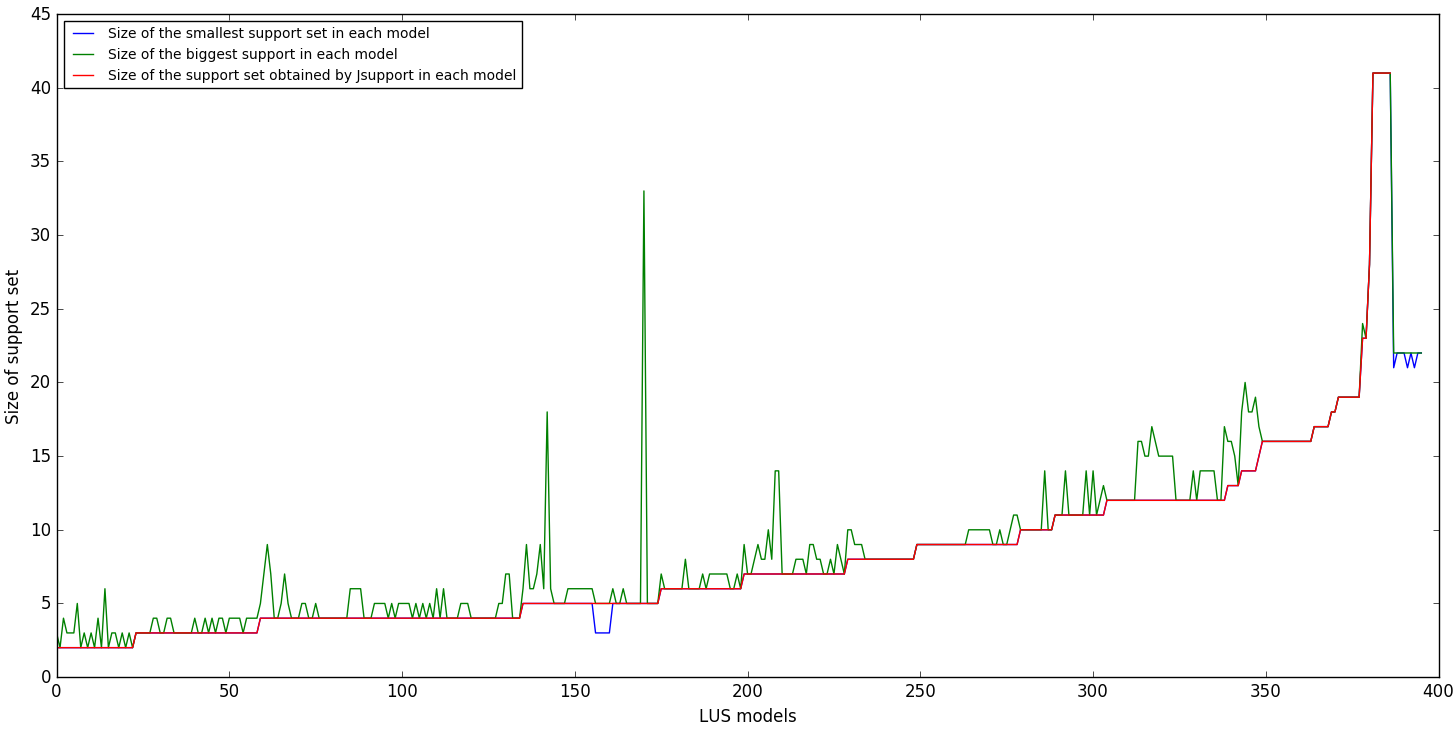
\includegraphics[width=\textwidth]{figs/minimality_analyses.png}
  \caption{\small{Minimality comparison}}\label{fig:minjsup}
\end{figure}

\vspace{6pt}
\noindent\fbox{%
    \parbox{\textwidth}{%
    Average size of sets computed by \texttt{JKind} is 8.55. And, average size of sets computed by \texttt{JSupport} is 7.60. 
    Therefore, in average, support sets computed by \texttt{JKind} are 88\% close to minimal.
    %  (1 - ((8.55 - 7.6)/ 7.6))  * 100 = 87.5%
    }%
}
 \vspace{9pt}
  
 
% RQ6: overall runtime in JSupport and different solvers
\textbf{RQ6.} In addition to overhead, it is also important to know how efficiently \texttt{JKind} performs on computing set of support in comparison with \texttt{JSupport}. Table~\ref{tab:eff-comp-jsup} compares overall runtime of support computation in different solvers and \texttt{JSupport}.


\begin{table}
  \centering
  \begin{tabular}{ |c||c|c|c|c| }
    \hline
     runtime (sec) & min & max & mean & stdev \\[0.5ex]
    \hline\hline
    JSupport & 2.381 & 165.157 & 21.533 & 23.533 \\[0.5ex]
    Z3   & 0.112 & 42.928 & 2.412 & 5.009 \\[0.5ex]
    Yices &   0.111  & 39.657   & 2.464 & 5.224 \\[0.5ex]
    SMTInterpol& 0.225 & 514.886 &  4.331 & 26.411 \\[0.5ex]
    MathSAT & 0.111 & 43.623 &  2.765 & 5.157 \\[0.5ex]
    \hline
  \end{tabular}
  \caption{\small{\texttt{JKind} runtime with \emph{-support} option in different solvers compared with \texttt{JSupport}}}
  \label{tab:eff-comp-jsup}
\end{table}


%For calculations, we considered all settings where both \texttt{K-induction} and \texttt{PDR} were activated
% then in for all 405 models in everything, we collected runtime info, then calculated min/max/avg/stdev between them
% in other words, there were 4 settings to be considered: z3_both, yices_both, mathsat_both, smtinterpol_both
For 405 models, runtime of support computation in the configurations where both \texttt{K-induction} and \texttt{PDR} were activated has been collected. Fig~\ref{fig:runtimez3} and Fig~\ref{fig:runtimeall} visualize the results.


%\begin{figure}
%\centering
%\begin{tabular}[c]{cc}
%    \begin{subfigure}[b]{0.20\textwidth}
%      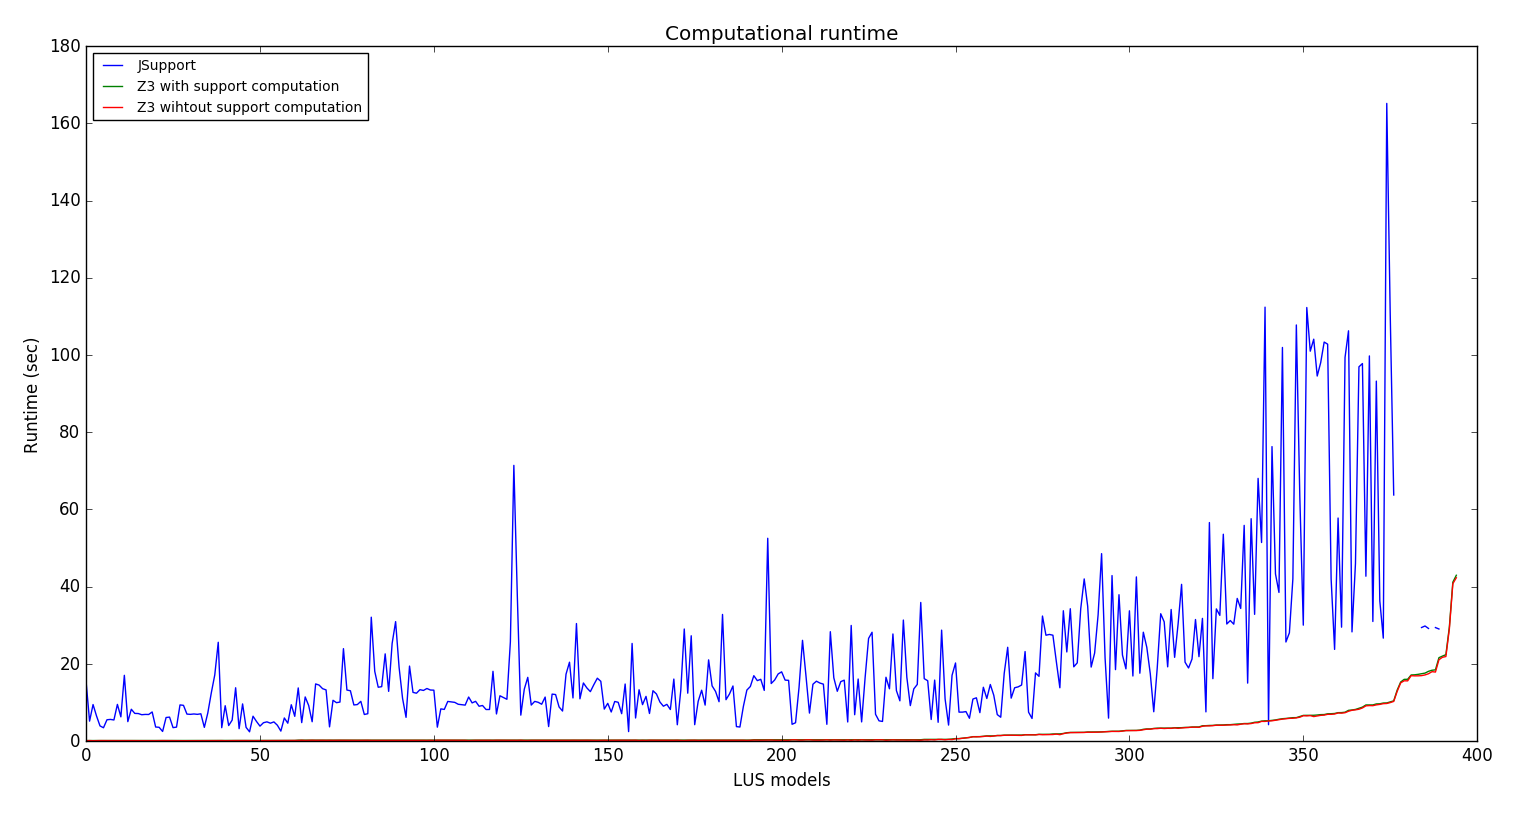
\includegraphics[width=\textwidth]{figs/figure_1.png}
%    \end{subfigure}&
%    \begin{subfigure}[b]{0.20\textwidth}
%      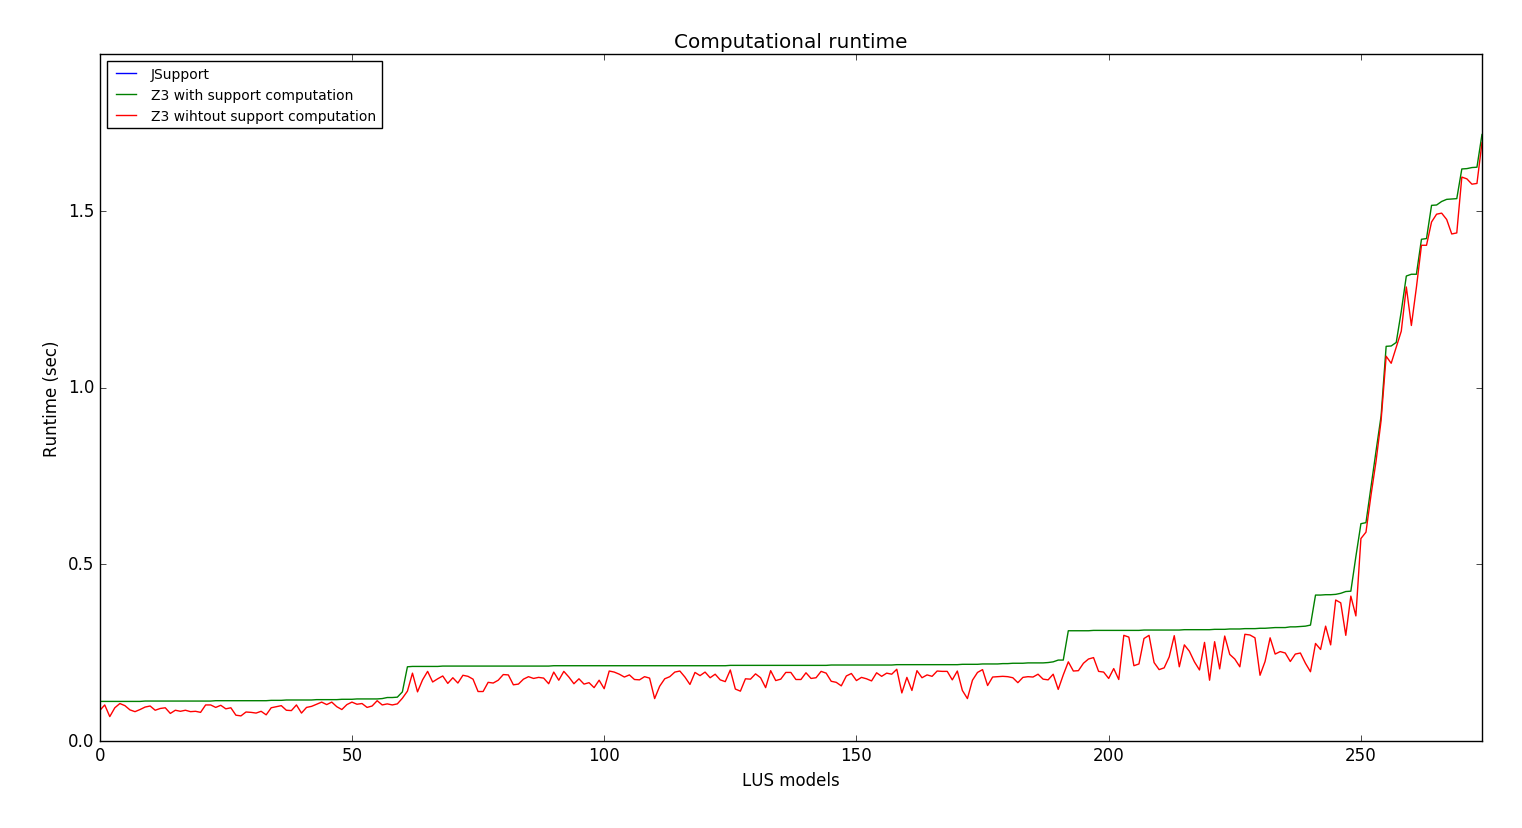
\includegraphics[width=\textwidth]{figs/figure_z3_zoom.png}
%    \end{subfigure}\\
%    \begin{subfigure}[b]{0.20\textwidth}
%      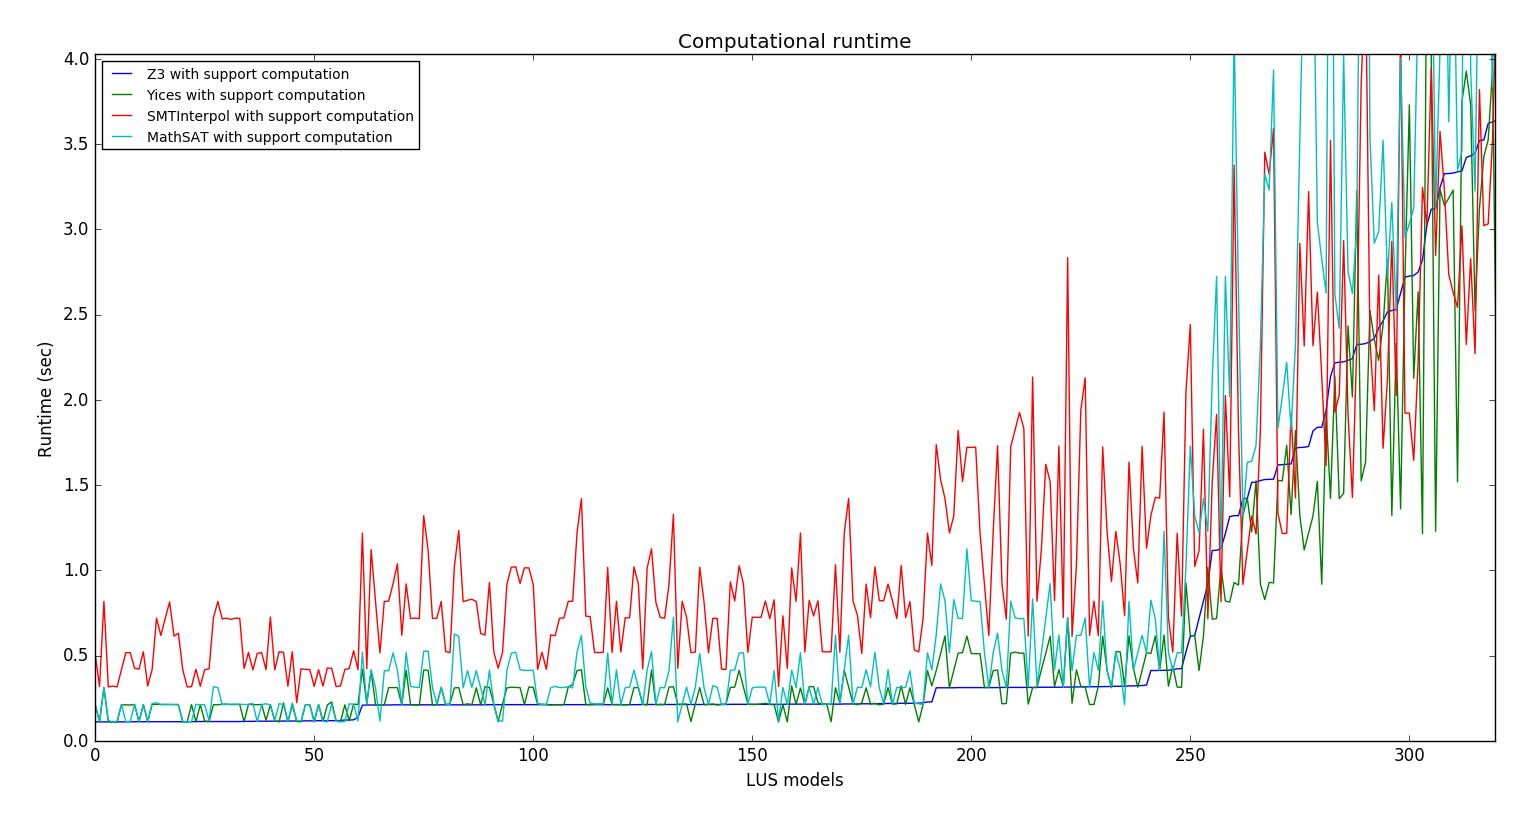
\includegraphics[width=\textwidth]{figs/solvers-support-zoom2.png}
%    \end{subfigure}&
%    \begin{subfigure}[b]{0.20\textwidth}
%      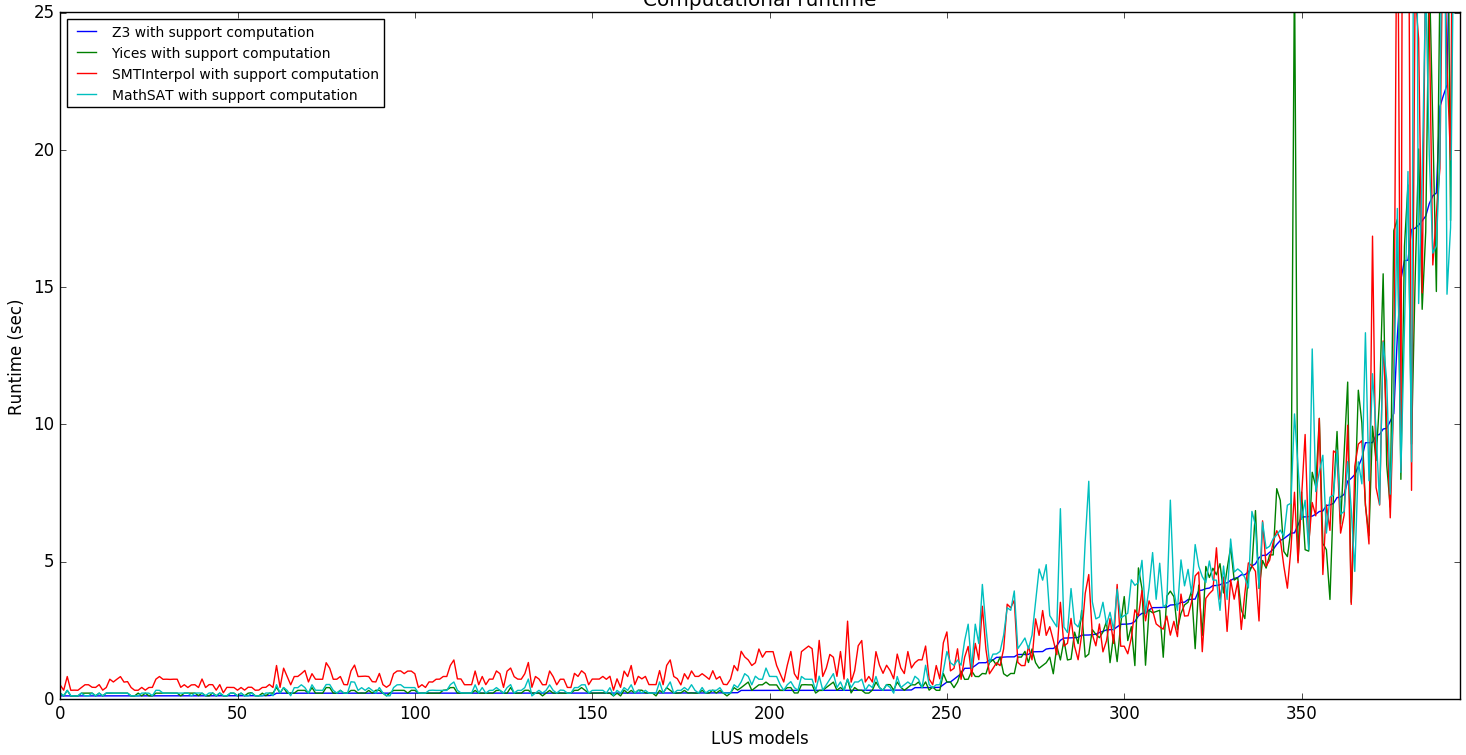
\includegraphics[width=\textwidth]{figs/solvers-support-zoom1.png}
%    \end{subfigure}
%  \end{tabular}
%\caption{\small{Runtime of support computation}}
%\label{fig:runtime}
%\end{figure}
\begin{figure}
  \centering
  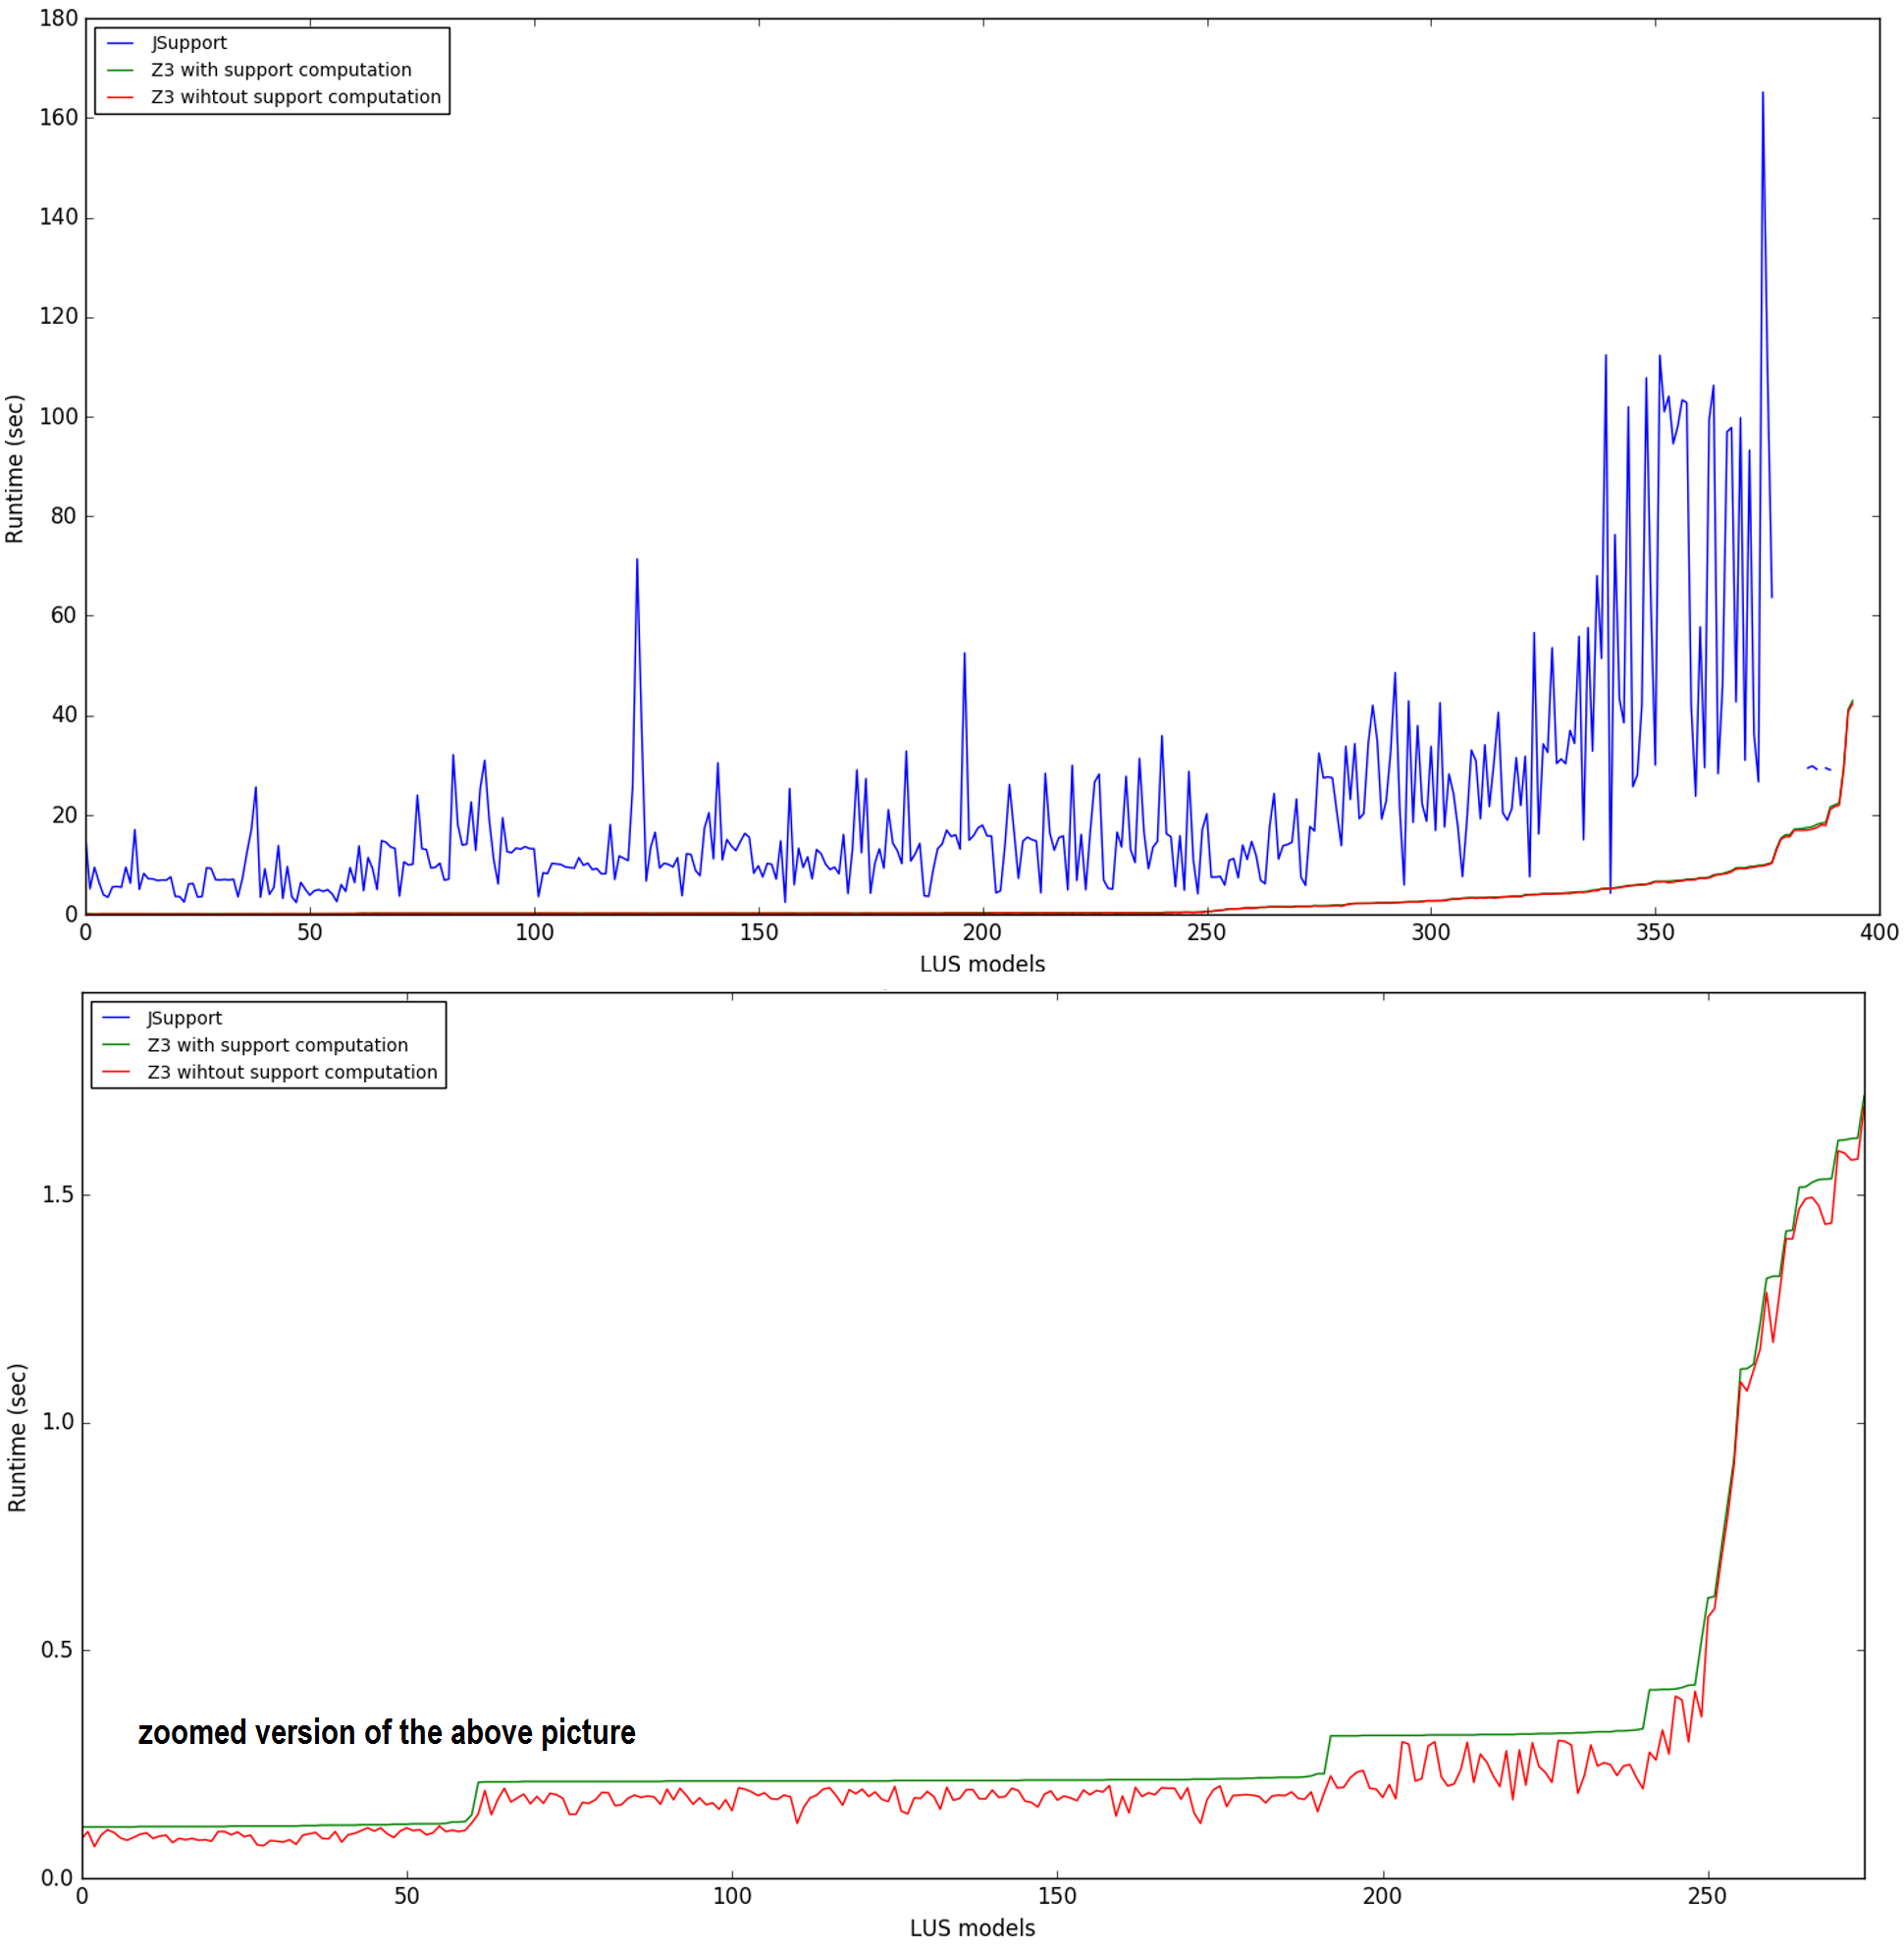
\includegraphics[width=\textwidth]{figs/runtimeZ3.png}
  \caption{\small{Runtime of support computation with \texttt{Z3} and \texttt{JSupport}}}\label{fig:runtimez3}
\end{figure}


\begin{figure}
  \centering
  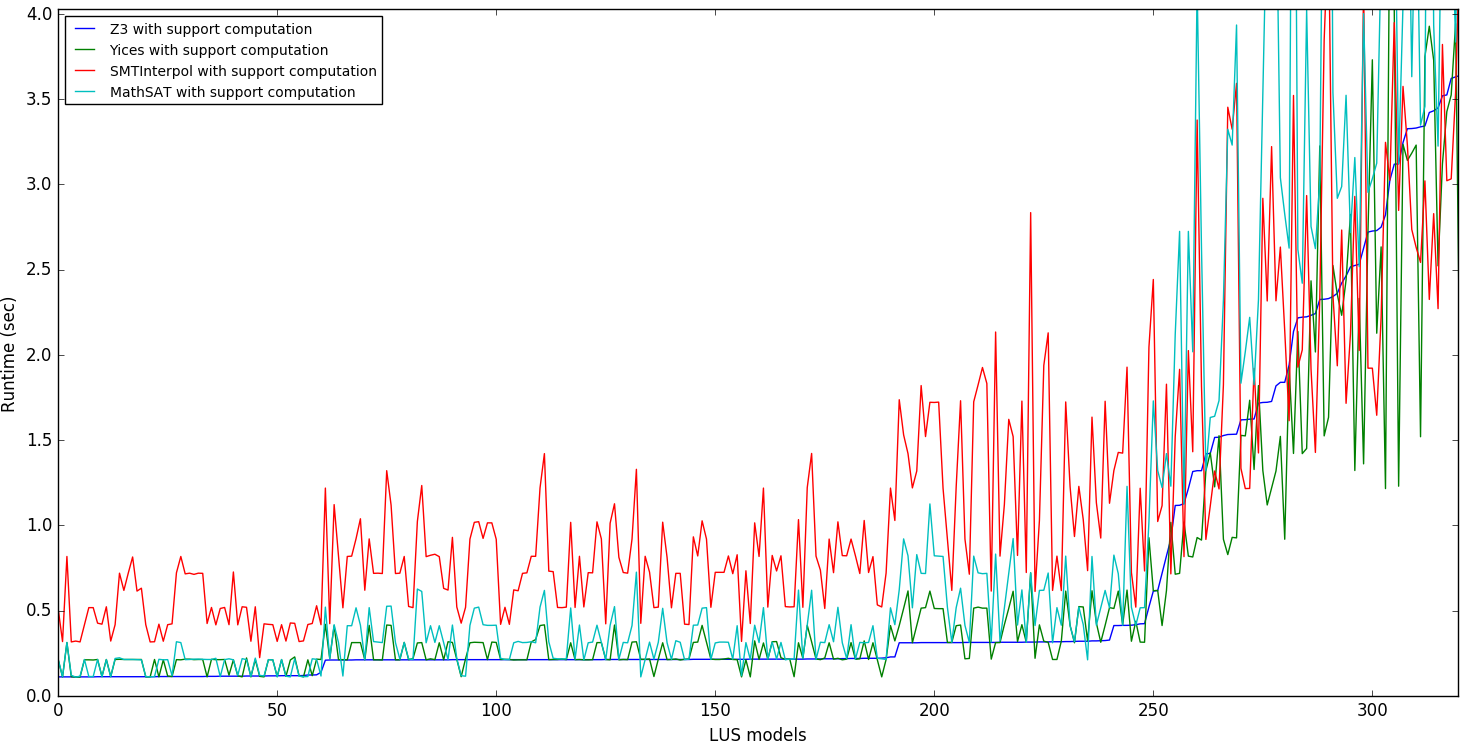
\includegraphics[width=\textwidth]{figs/runtimeAll.png}
  \caption{\small{Runtime of support computation with all solvers}}\label{fig:runtimeall}
\end{figure}


\vspace{6pt}
\noindent\fbox{%
    \parbox{\textwidth}{%
        Time-efficiency of computing support set in \texttt{JKind} is not quite solver-dependent. However, SMTInterpol works less efficiently in comparison with others. 
    }%
}
\noindent\fbox{%
    \parbox{\textwidth}{%
        Support computation by \texttt{JSupport} is much more time-consuming than \texttt{reduce-support} engine.
    }%
}
 \vspace{9pt}

\section{Conclusions \& Future Work}
\label{sec:conc}
The idea of extracting a minimal IVC for a given property, and applications for doing so was recently introduced in \cite{Ghass16}.  However, a single IVC often does not provide a complete picture of the traceability from a property to a model.  In this paper,
we have addressed the problem of extracting {\em all minimal} IVCs. We have shown
the correctness and completeness of our method and algorithm.  In addition, we have a substantial evaluation that shows that the practicality and efficiency of our technique.

Our method is inspired by a recent work in the domain of satisfiability analysis \cite{marco2016fast}. One interesting future direction is to devise similar MIVC enumeration algorithms based on other studies on MUSes extraction such as \cite{nadel2014accelerated}.  We are also looking into improving our implementation by using more  efficient methods for the \isadeq ~and \getivc ~modules used by our algorithm. Another interesting direction is to parallelize the enumeration process: it is certainly possible to ask for multiple distinct maximal models to be solved in parallel.
%, though this may result in unnecessary work performed by some of the parallel solvers.

We also plan to investigate additional applications of the idea.  When performing {\em compositional verification}, the All-IVCs technique may be able to determine {\em minimal component sets} within an architecture that can satisfy a given set of requirements, which may be helpful for design-space exploration and synthesis. Finally, we are interested in adapting the notion of (all) validity cores for \emph{bounded} model checking for quantifying how much of models have been explored by bounded analysis. 
%ACKNOWLEDGMENTS are optional
\vspace{0.05in}
%\textbf{Acknowledgments:}
%We thank XXXX

\bibliographystyle{splncs03}
\bibliography{biblio}

\end{document}
